\chapter{Design}
This chapter provides an in-depth description of the system architecture and its individual components, based heavily on the conclusions drawn from Chapter \ref{chap:analysis} \nameref{chap:analysis}.

\section{Architecture Design}
The system can be divided into multiple main parts\footnote{Note: These do not necessarily overlap with the modular aspects of the system.}, the highest-level of division can be into a basic  three-layered architecture containing these three layers:
\begin{itemize}
\item Client layer
\item Business layer
\item Data layer (often referred to as Storage layer)
\end{itemize}

Figure ~\ref{fig:layer-arch} shows these three layers and the components belonging in each. Due to the high modularity requirements of the system, only most of the Business layer belongs into the core system, the Client and Data layers are to be easily interchangeable and therefore will be part of the sample implementation. A more concrete version of the tiered architecture for the full sample implementation can be seen in Figure ~\ref{fig:s-impl-arch}.

\begin{figure}[H]
	\centering
	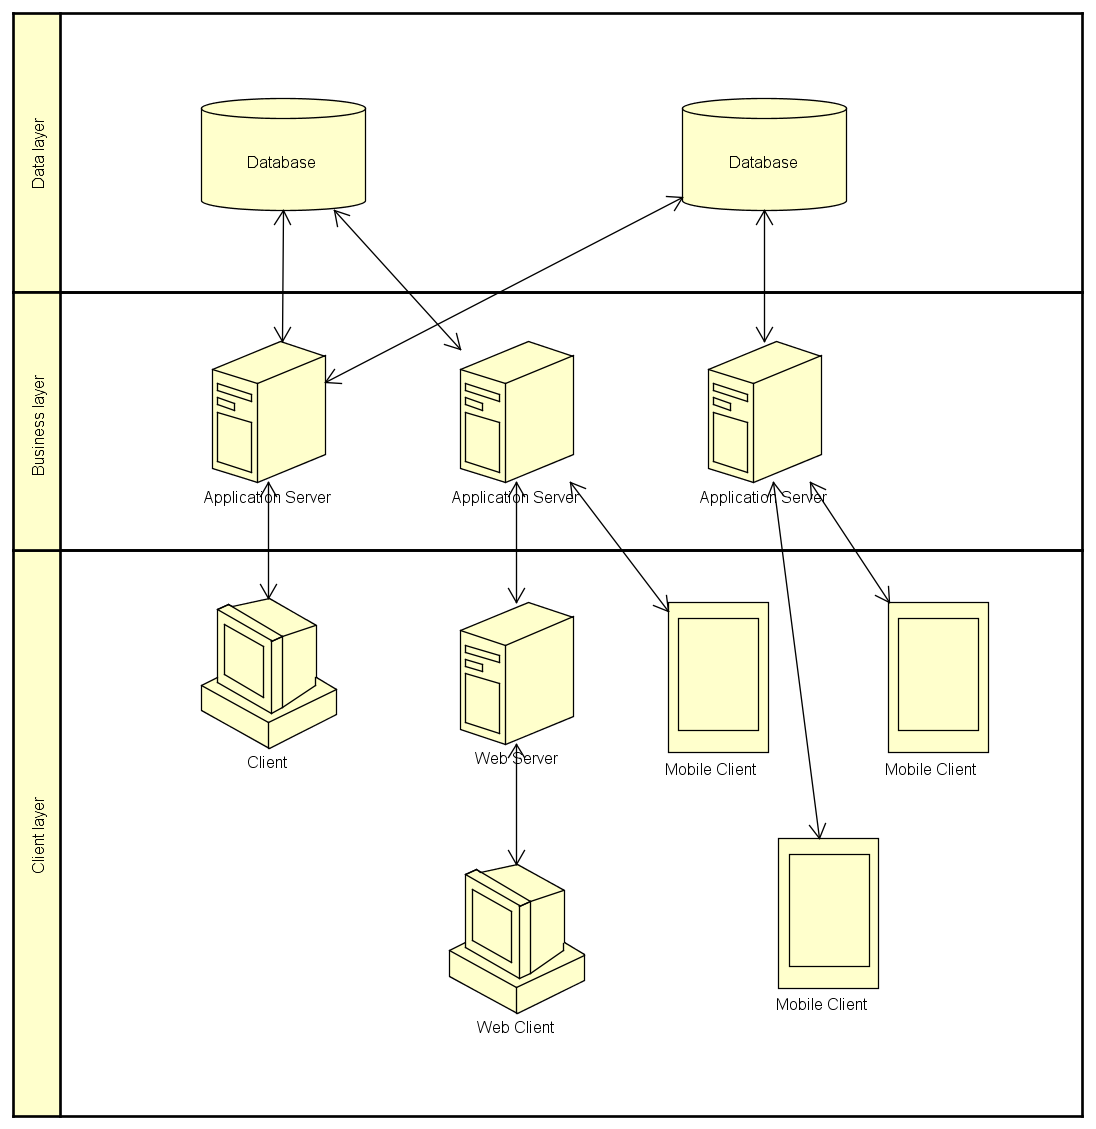
\includegraphics[width=1\textwidth]{figures/03_design/layer-arch}
    \caption{Three layered basic system architecture}
    \label{fig:layer-arch}
\end{figure}

\begin{figure}[H]
	\centering
	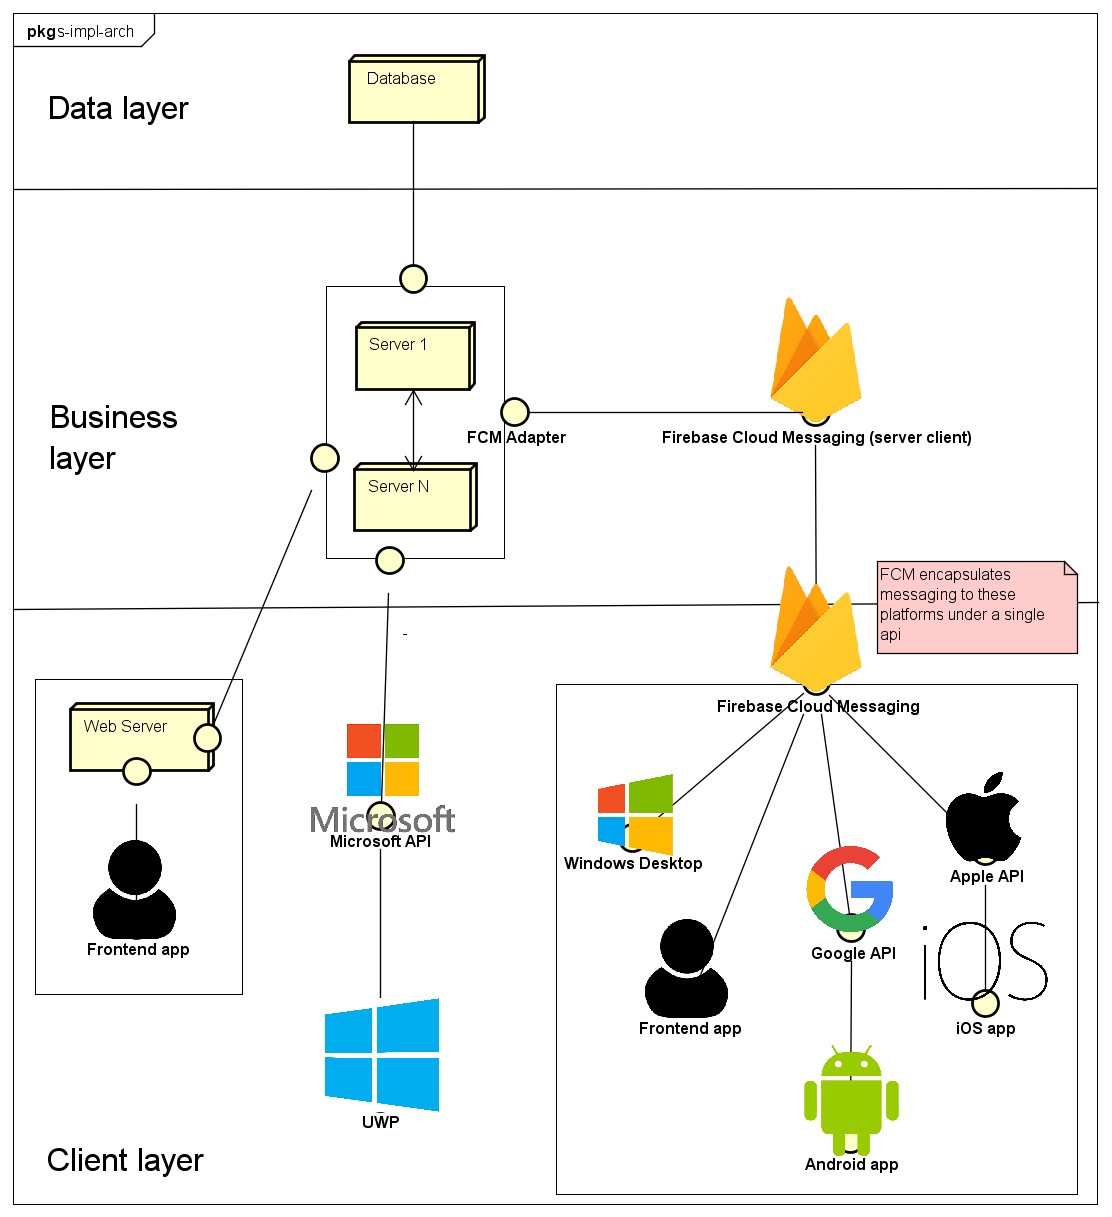
\includegraphics[width=1\textwidth]{figures/03_design/s-impl-arch}
    \caption{Three layered system architecture for sample implementation}
    \label{fig:s-impl-arch}
\end{figure}

\subsection{Data Layer}
The data layer will be used to persistently store data regarding how messages should be handled and how they are to be delivered to their intended recipient. After analysing the necessary requirements, the data to be stored was divided into the following entities.
\begin{itemize}
\item \textbf{Group:} The Group entity represents a collection of Users, aggregated for some reason, eg. a topic in a publish/subscribe pattern.
\item \textbf{User:} The User entity represents an end user of the application using the system. A User can belong to Groups and has Devices.
\item \textbf{Device:} The Device entity represents an end device onto which messages will be delivered. Every Device belongs to a User and is on a certain Platform.
\item \textbf{Platform:} The Platform entity represents the platform on which a Device is running and therefore determines how a message is to be delivered to that Device, eg. Android, iOS, FCM, etc.
\end{itemize}

Due to the high modularity design required of the system, the core of the system will only contain interfaces and instructions for the implementation of a data layer.

\subsubsection{Sample Implementation Data Layer}
In the sample implementation, which is part of this thesis, a relational database system will be used. The Object-Relational Mapping (ORM) implementation design of the data layer interface can be seen in Figure ~\ref{fig:orm}

\begin{figure}[H]
	\centering
	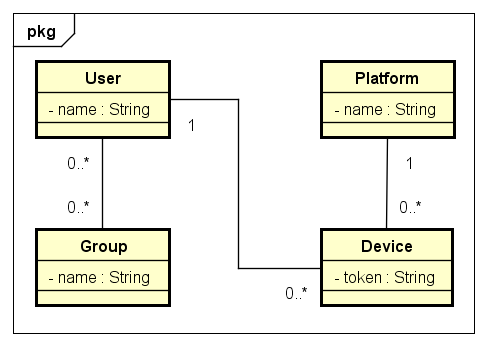
\includegraphics[width=0.6\textwidth]{figures/03_design/orm}
    \caption{Sample Implementation ORM Data Layer design}
    \label{fig:orm}
\end{figure}

\subsection{Business Layer}
The business layer, also commonly known as the business logic layer, is where all the main functions of the system are done. In this case, it is where messages are sorted received, sorted and passed along to their respective adapters\footnote{More on adapters in Section \ref{sec:adapters}} to be sent to their target end devices. 

Figure ~\ref{fig:msg-flow} shows a simplified representation of the flow of a message through the business layer. The message starts at the point from where it is sent, after being received through the system's API it is processed and passed to the MessagingService, which communicated with the Data layer to find information on the groups, users, devices and platforms the message is to be sent to. After this, the message is passed the AdapterService, which then delegates it to the respective adapters of the devices it is meant to be sent to and finally, the message is sent out to the end devices.

\begin{figure}[H]
	\centering
	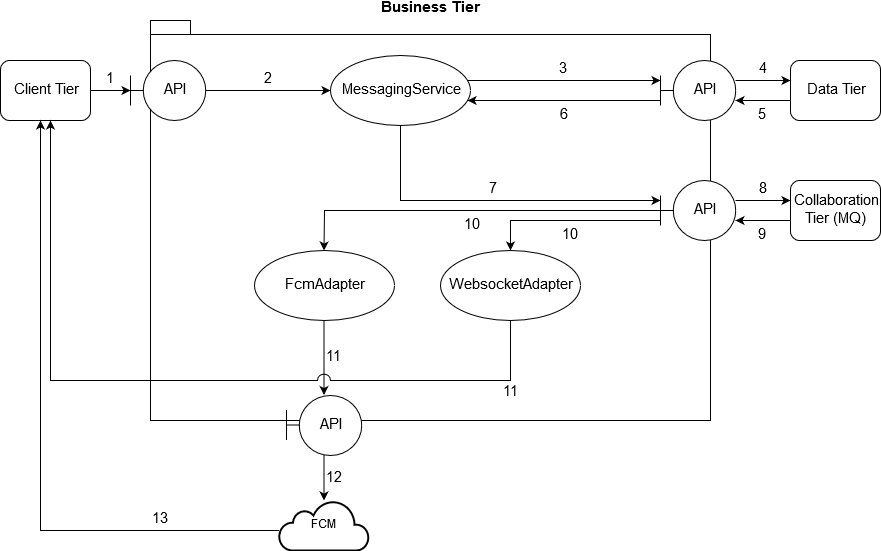
\includegraphics[width=0.8\textwidth]{figures/03_design/msg-flow}
    \caption{Flow of a message through the Business layer}
    \label{fig:msg-flow}
\end{figure}

\subsection{Client Layer}
The client layer includes all client libraries and applications that can receive and/or send messages from/to the system. Because the client layer must be designed with high modularity in mind, none of it is part of the main system and the specifics of its API depend on the individual adapters\footnote{More on adapters in Section \ref{sec:adapters}} that go with it.

\subsubsection{Sample Implementation Client Layer}
The sample implementation that is part of this thesis will include an implementation of the client layer, aka the client libraries, for the platforms stated in Section \ref{sec:s-impl-func-req} \nameref{sec:s-impl-func-req}.
\subsubsection*{Java}
The client library for the Java platform will be a Java Archive (JAR) file, that can be included in a Java application's classpath and provides interfaces to send and receive messages to and from the system, respectively. It will be independent of any framework, such as Spring, so that it works with any Java application.

With real-time communication in mind, the design of the client library was made using an Event Driven architectural pattern. Figure \ref{fig:java-client-classes} shows an overview of the classes the library will contain. The most important class being \textit{MsgrClient}, which is the main point of interaction for the user. It contains methods for sending messages and adding or removing message listeners. Message listeners will be user created implementations of the \textit{IMessageListener} interface. Data container classes are not important to the overall architecture design, they serve simply as POJOs (Plain Old Java Objects) that envelop data, along with providing getters and setters, in order to pass the data between components in a simple, encapsulated object-oriented manner. These include classes such as \textit{Message}, \textit{User}, etc.

\begin{figure}[H]
	\centering
	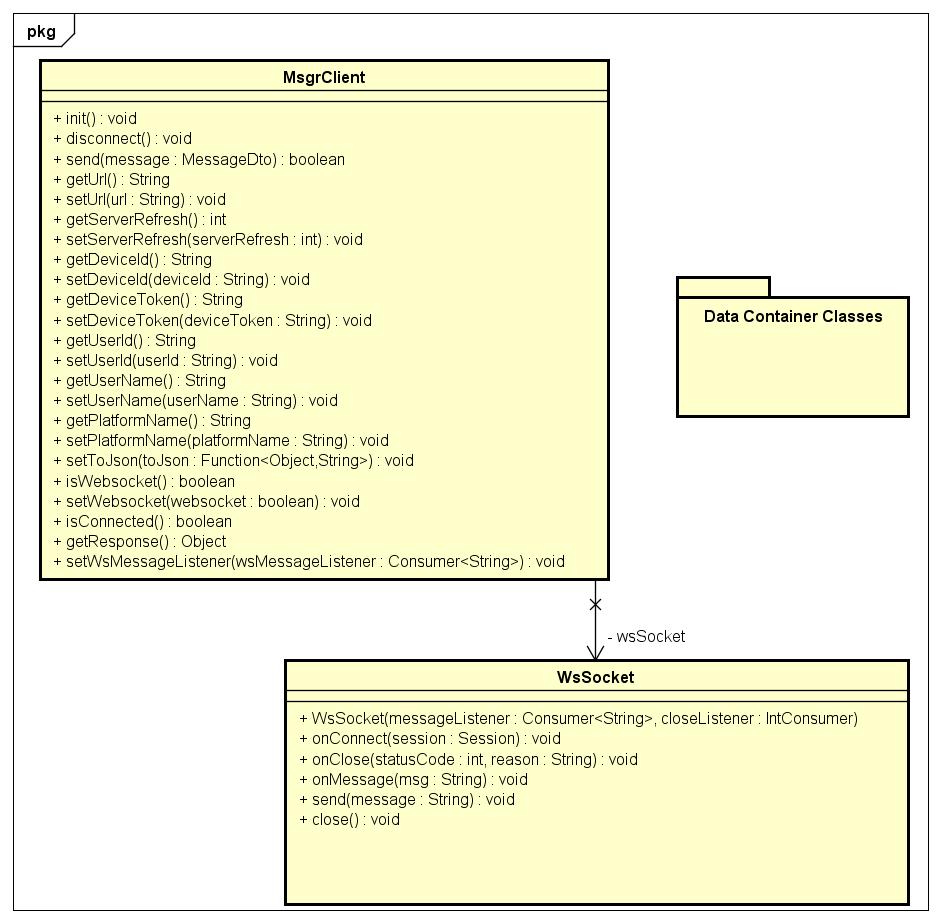
\includegraphics[width=0.8\textwidth]{figures/03_design/java-client-classes}
    \caption{Design of the main class components of the Java client library}
    \label{fig:java-client-classes}
\end{figure}

\subsubsection*{Android \& iOS}
The Android and iOS clients will be simple applications for each platform, using Google's Firebase Cloud Messaging (FCM) client libraries, which are provided for both the Android\cite{fcm-android-client} and iOS\cite{fcm-ios-client} platforms.

\subsubsection*{Web}
The Web client will be a simple HTML, CSS and Javascript application using Google's FCM Javascript client library, which supports the majority of modern browsers (versions: Chrome 50+, Firefox 44+, Opera Mobile 37+)\cite{fcm-web-client}.

\section{Modularity Design}

A critical part of the requirements put onto the system is its high flexibility and adaptability, based on high modularity. For this reason, the system has been designed with maximum modularity in mind. In order to achieve this, the main system is contained in a Core module, which will be the basis for any full applications with the system. Functionality and components that may be interchanged depending on the applications' needs will be contained in modules, which will be added to the full application as further dependencies (side-to-side with the Core module). An example of an application with different modules can be seen in Figure \ref{fig:s-impl-comps}, which shows the module structure that will be used in the Sample Implementation.

\begin{figure}[H]
	\centering
	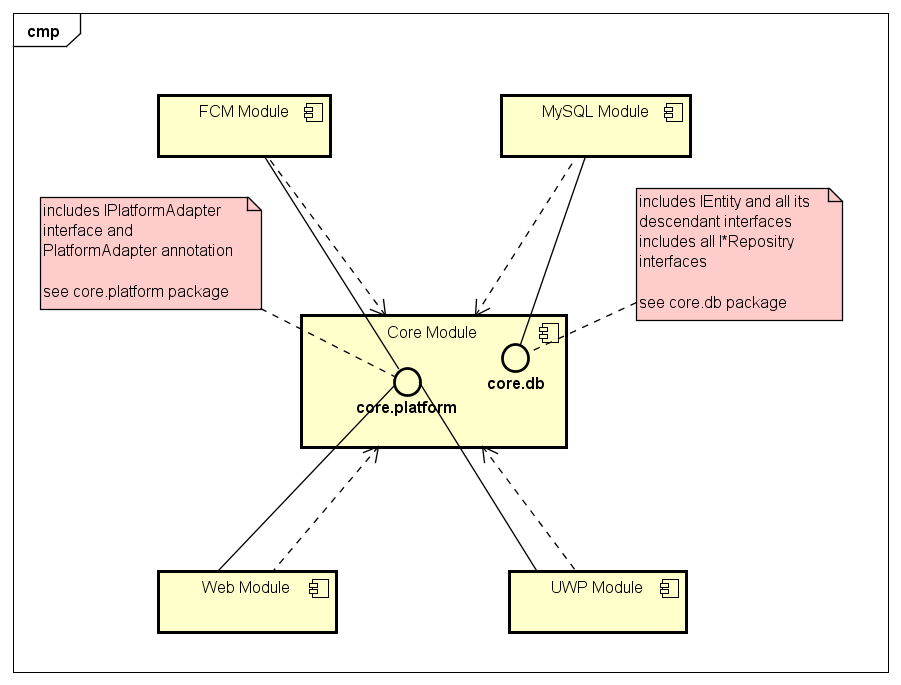
\includegraphics[width=0.8\textwidth]{figures/03_design/s-impl-comps}
    \caption{Module structure design of sample implementation}
    \label{fig:s-impl-comps}
\end{figure}

\subsection{Core Module}
The Core module, or Core library, is the heart of the entire system. The Core module provides the interfaces needed for other modules to implement and Spring Managed Beans (from now on referred to simply as Beans). Beans are objects whose lifecycle is managed by the Spring's IoC Container's Application Context, which means the Spring Container initializes and configures them and where needed, allows them to be injected\cite{spring-beans}. These Beans provide the main business logic of the application as well as manage the cooperation between all modules. The design of these interactions is further elaborated upon in the following sections.

\subsection{Database Modularity}
The system's access to the data layer has been designed in a fully modular way, so that the end deployment is not dependent on any one type or provider of database. The result of this effort for maximum freedom and interchangeability are the interfaces in the \textit{core.db} package, as seen in Figure \ref{fig:core-db-module}.

\begin{figure}[!ht]
	\centering
	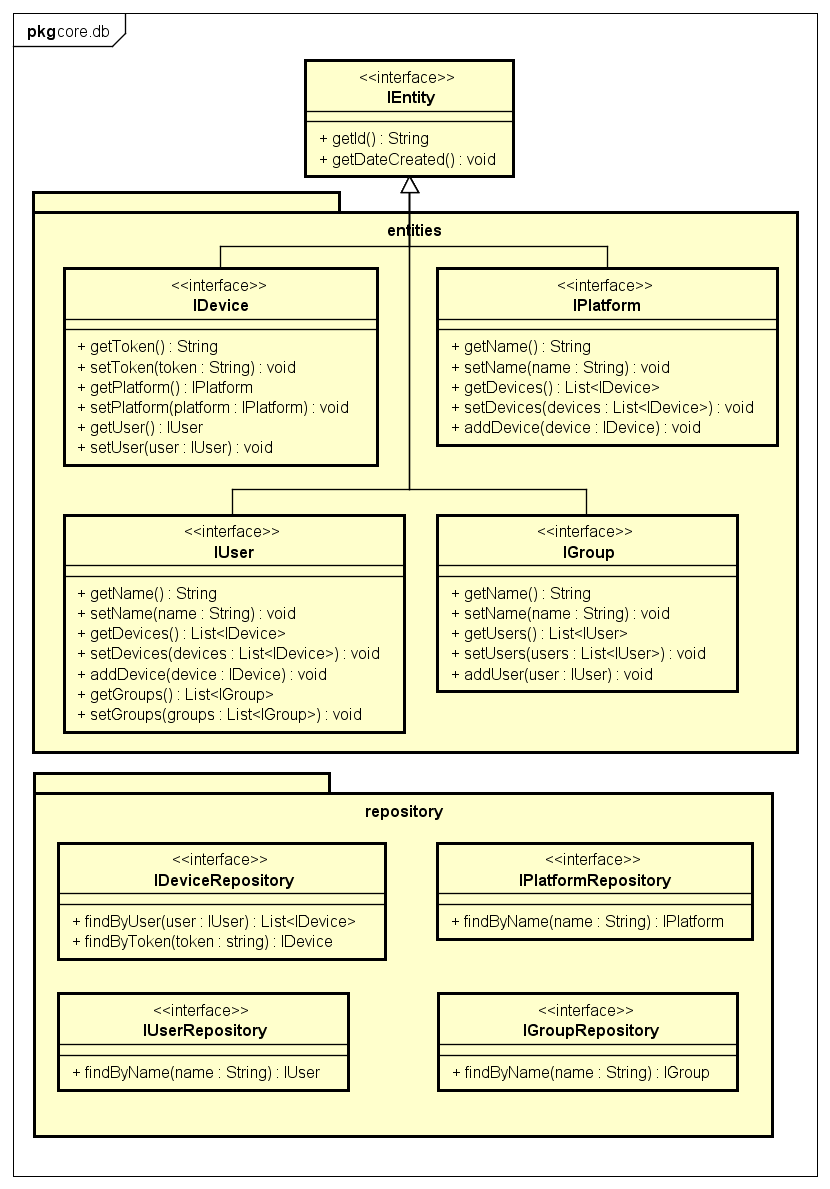
\includegraphics[width=0.95\textwidth]{figures/03_design/core-db-module}
    \caption{Interfaces for database modules in the \textit{core.db} package}
    \label{fig:core-db-module}
\end{figure}

Any module that wishes to implement access to a database must create JPA Entities implementing the entity interfaces and create interfaces that extend the repository interfaces and extend Spring Data's \textit{CrudRepository} interface. This will indicate to the Spring Context to instantiate repository Beans based on these interfaces\cite{spring-repos}, which the Context will then inject into the Beans where they are used.

\subsection{Platform Modularity}
One of the key features of the system is its multi-platform support. In order to be able to support the widest possible range of platforms, the platform portion of the system had to be designed with complete modularity in mind. The results of the design choices made based on these requirements led to the creation of the \textit{IPlatformAdapter} interface and \textit{@PlatformAdapter} annotations, which can be seen in more detail in Figure \ref{fig:core-platform-module}.

\begin{figure}[!ht]
	\centering
	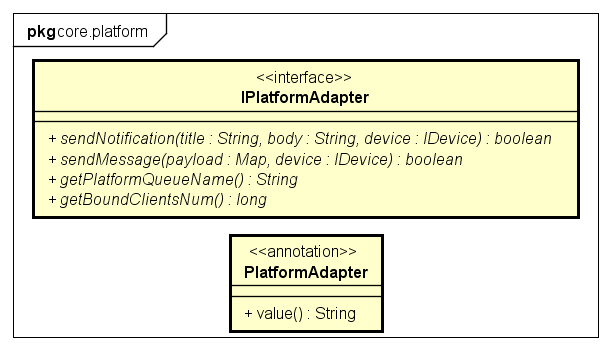
\includegraphics[width=0.95\textwidth]{figures/03_design/core-platform-module}
    \caption{Interfaces for platform modules in the \textit{core.platform} package}
    \label{fig:core-platform-module}
\end{figure}

Any module that wishes to implement support for a new platform must contain at least one Bean implementing the \textit{IPlatformAdapter} interface and annotate it with the \textit{@PlatformAdapter} annotation, which takes the platform's name as a parameter.

\subsubsection{Adapters}\label{sec:adapters}
Platform Adapters are Spring Managed Beans that implement the Core module's \textit{IPlatformAdapter} interface and are annotated with the \textit{@PlatformAdapter} annotation, which takes the platform's name as a parameter. 

Adapters will be automatically found at system startup by the Core module's \textit{AdapterService} using Spring's Application Context and registered based on the platform's name, as specified in the \textit{@PlatformAdapter} annotation. After which whenever a message is sent to a device through the \textit{MessagingService}, the \textit{AdapterService} will provide the Adapter needed to send message for the platform of that device to the \textit{MessagingService}, which will then use it to send the message. The sequence of these events including an example message being sent can be seen illustrated in Figure \ref{fig:adapter-flow}

\begin{figure}[!ht]
	\centering
	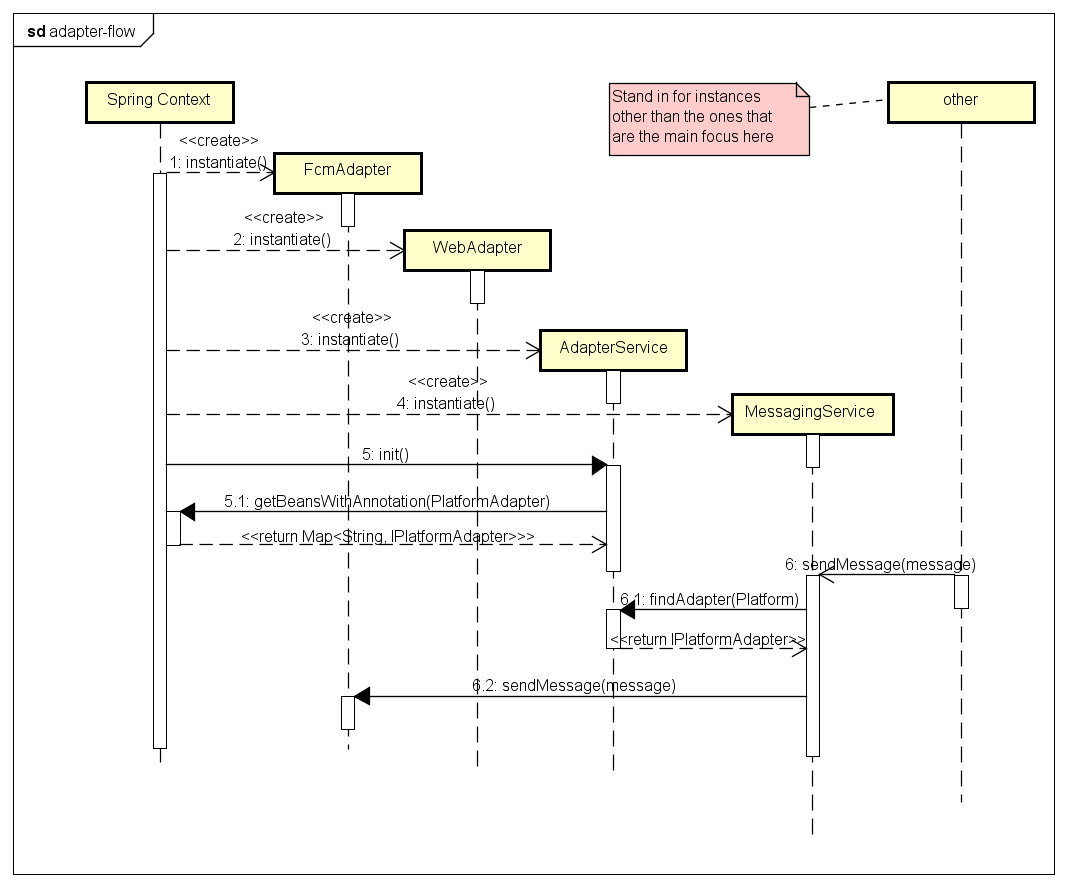
\includegraphics[width=0.9\textwidth]{figures/03_design/adapter-flow}
    \caption{Sequence diagram indicating the resolution process of Adapters}
    \label{fig:adapter-flow}
\end{figure}